\begin{textblock}{15.}(0., -4.)
    \begin{tikzpicture}
        %%% Definitions
        %% Mathematical constants
        \def \INVERSESQRTTWO {0.7071067811865475}
        \def \NWAVEFORMSAMPLES {50}

        %% Colors
        \def \INELASTICHIGHCOLOR {brown}
        \def \INELASTICLOWCOLOR {red}

        %% Incoming EM wave
        \def \AMPLITUDE {0.4}
        \def \WAVEFORMLENGTH {3.}
        \def \INWAVESTART {0.}
        \def \INWAVELENGTH {0.5}

        %% Outgoing EM wave
        \def \OUTWAVELENGTHHIGH {1.0}
        \def \OUTWAVELENGTHLOW {1.5}

        %% Atom
        \def \ELECTRONRADIUS {0.3}
        \def \ELECTRONCOLOR {gray}

        \def \ORBITALINRADIUS {1.5}
        \def \ORBITALMIDRADIUS {2.2}
        \def \ORBITALOUTRADIUS {3.2}

        \def \ATOMX {5.}
        \coordinate (ATOMPOSITION) at (\ATOMX, 0.);

        %% Nucleus
        \def \NUCLEUSRADIUS {0.4}

        %%% Drawing
        %% Atom
        % Nucleus
        \draw [very thick, black, dashed] (ATOMPOSITION) circle [radius = \NUCLEUSRADIUS];

        % Orbitals
        \draw [very thick, black] (ATOMPOSITION) circle [radius = \ORBITALINRADIUS];
        \draw [very thick, black] (ATOMPOSITION) circle [radius = \ORBITALMIDRADIUS];
        \draw [very thick, black] (ATOMPOSITION) circle [radius = \ORBITALOUTRADIUS];

        % Electrons
        % Inner electrons
        \visible<1-2,5->{
            \draw [very thick, black, fill=\ELECTRONCOLOR] ($ (ATOMPOSITION) + \ORBITALINRADIUS*(0,1)$) circle [radius = \ELECTRONRADIUS];
        }
        \visible<3>{
            \draw [very thick, black, fill=\ELECTRONCOLOR] ($ (ATOMPOSITION) + \ORBITALOUTRADIUS*(0,1)$) circle [radius = \ELECTRONRADIUS];
        }
        \visible<4>{
            \draw [very thick, black, fill=\ELECTRONCOLOR] ($ (ATOMPOSITION) + \ORBITALMIDRADIUS*(0,1)$) circle [radius = \ELECTRONRADIUS];
        }
        \draw [very thick, black, fill=\ELECTRONCOLOR] ($ (ATOMPOSITION) + \ORBITALINRADIUS*(0,-1)$) circle [radius = \ELECTRONRADIUS];

        % Outer electrons
        \draw [very thick, black, fill=\ELECTRONCOLOR] ($ (ATOMPOSITION) + \INVERSESQRTTWO*\ORBITALMIDRADIUS*(1,1)$) circle [radius = \ELECTRONRADIUS];
        \draw [very thick, black, fill=\ELECTRONCOLOR] ($ (ATOMPOSITION) + \INVERSESQRTTWO*\ORBITALMIDRADIUS*(1,-1)$) circle [radius = \ELECTRONRADIUS];
        \draw [very thick, black, fill=\ELECTRONCOLOR] ($ (ATOMPOSITION) + \INVERSESQRTTWO*\ORBITALMIDRADIUS*(-1,1)$) circle [radius = \ELECTRONRADIUS];
        \draw [very thick, black, fill=\ELECTRONCOLOR] ($ (ATOMPOSITION) + \INVERSESQRTTWO*\ORBITALMIDRADIUS*(-1,-1)$) circle [radius = \ELECTRONRADIUS];

        %% Incoming EM wave
        \visible<2>{
            \draw [very thick, \ORANGE, domain=\ATOMX-\ELECTRONRADIUS-\WAVEFORMLENGTH:\ATOMX-\ELECTRONRADIUS, samples=\NWAVEFORMSAMPLES] plot (\x, {\AMPLITUDE*sin(\WAVEFORMLENGTH/\INWAVELENGTH*2*pi/4*\x r) + \ORBITALINRADIUS});
        }

        %% Transitions
        % Excitation
        \visible<3>{
            \draw [->, very thick, black] (\ATOMX, \ORBITALINRADIUS) -- (\ATOMX, \ORBITALOUTRADIUS-\ELECTRONRADIUS);
        }
        \visible<4>{
            \draw [->, very thick, black] (\ATOMX, \ORBITALOUTRADIUS) -- (\ATOMX, \ORBITALMIDRADIUS+\ELECTRONRADIUS);
        }
        \visible<4->{
            \draw [very thick, \INELASTICHIGHCOLOR, domain=\ATOMX:\ATOMX+\WAVEFORMLENGTH, samples=\NWAVEFORMSAMPLES] plot (\x, {\AMPLITUDE*sin(\WAVEFORMLENGTH/\OUTWAVELENGTHHIGH*2*pi/4*\x r) + \ORBITALMIDRADIUS + 0.5*(\ORBITALOUTRADIUS-\ORBITALMIDRADIUS)});
        }
        \visible<5->{
            \draw [->, very thick, black] (\ATOMX, \ORBITALOUTRADIUS) -- (\ATOMX, \ORBITALMIDRADIUS);
            \draw [->, very thick, black] (\ATOMX, \ORBITALMIDRADIUS) -- (\ATOMX, \ORBITALINRADIUS+\ELECTRONRADIUS);
            \draw [very thick, \INELASTICLOWCOLOR, domain=\ATOMX:\ATOMX+\WAVEFORMLENGTH, samples=\NWAVEFORMSAMPLES] plot (\x, {\AMPLITUDE*sin(\WAVEFORMLENGTH/\OUTWAVELENGTHLOW*2*pi/4*\x r) + \ORBITALINRADIUS + 0.5*(\ORBITALMIDRADIUS-\ORBITALINRADIUS)});
        }
    \end{tikzpicture}
\end{textblock}

\begin{textblock}{5.}(8., -6.)
    \begin{center}
        \begin{tabular}{ll}
        & Atom  \\
        \hline
        Res. Energy & $\unit[10^{0}]{eV}$ \\
        Res. Width & $> \unit[10^{-7}]{eV}$ \\
        System mass $\times c^2$ & $\unit[10^{9}]{eV}$ \\
        \end{tabular}
    \end{center}
\end{textblock}

\begin{textblock}{7.}(8.5, -1.5)
    \begin{itemize}
    \visible<2->{
        \item \textbf{Photon source}: \\ 'conventional' light sources, \textbf{laser}
    }
    \visible<6>{
        \item \textbf{Photon spectroscopy}: \\
        prisms, diffraction grids
    }
    \end{itemize}
\end{textblock}

\begin{textblock}{6.}(8.5, 3.2)
    \visible<6>{
        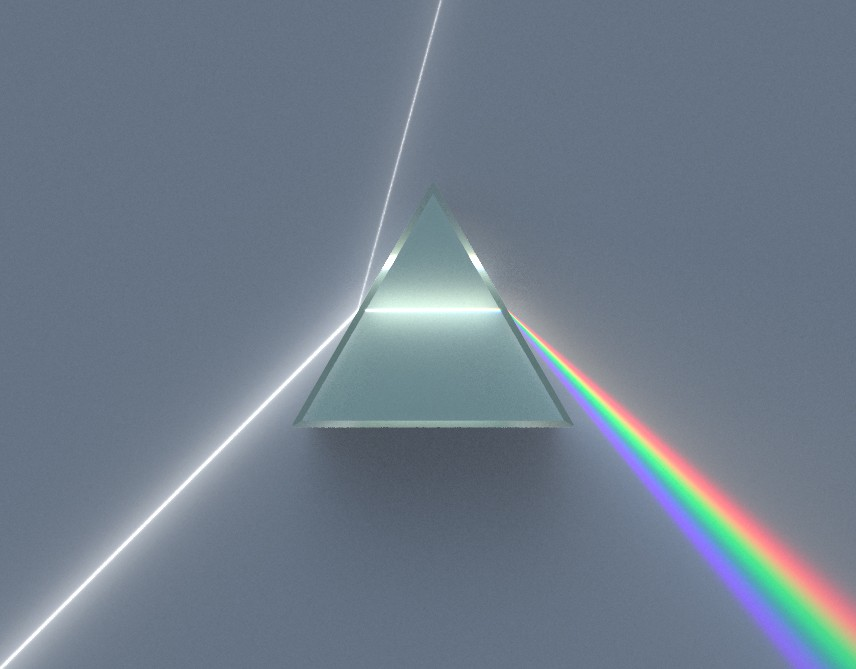
\includegraphics[width=\textwidth]{figures/prism.jpg}
    }
\end{textblock}